\section{Encoder and CANivore Set Up and Motor Testing}
\resetassemblysteps

\begin{partsbox}
\begin{minipage}[t]{\linewidth}
\vspace{0pt}
\begin{itemize}
\item
  PDP and Swerve Module Assembly set up
\item
  \href{https://store.ctr-electronics.com/products/canivore?_pos=1\&_psq=CANiv\&_ss=e\&_v=1.0}{CANivore
  Bus Expansion} --
  \href{https://ctre.download/files/user-manual/CANivore\%20User's\%20Guide.pdf}{User
  Guide} --
  \href{https://github.com/CrossTheRoadElec/Device-CADs/raw/master/CANIVORE_CAD/CANivore.zip}{CAD/Drawings}
\end{itemize}
\end{minipage}
\end{partsbox}

\assemblystep{Connect the First Encoder to the CANivore}
Press the red button on the 120A circuit breaker to turn off the
circuit. You will see the yellow lever rotate out if it is not already.
Take one pair of the green and yellow signal wires from one of the
encoders and either remove the jumper connector or trim and strip the
wires. While pressing the tan button on the CANivore unit, insert the
cables into the correctly labeled slot.

\begin{figure}[H]
\centering
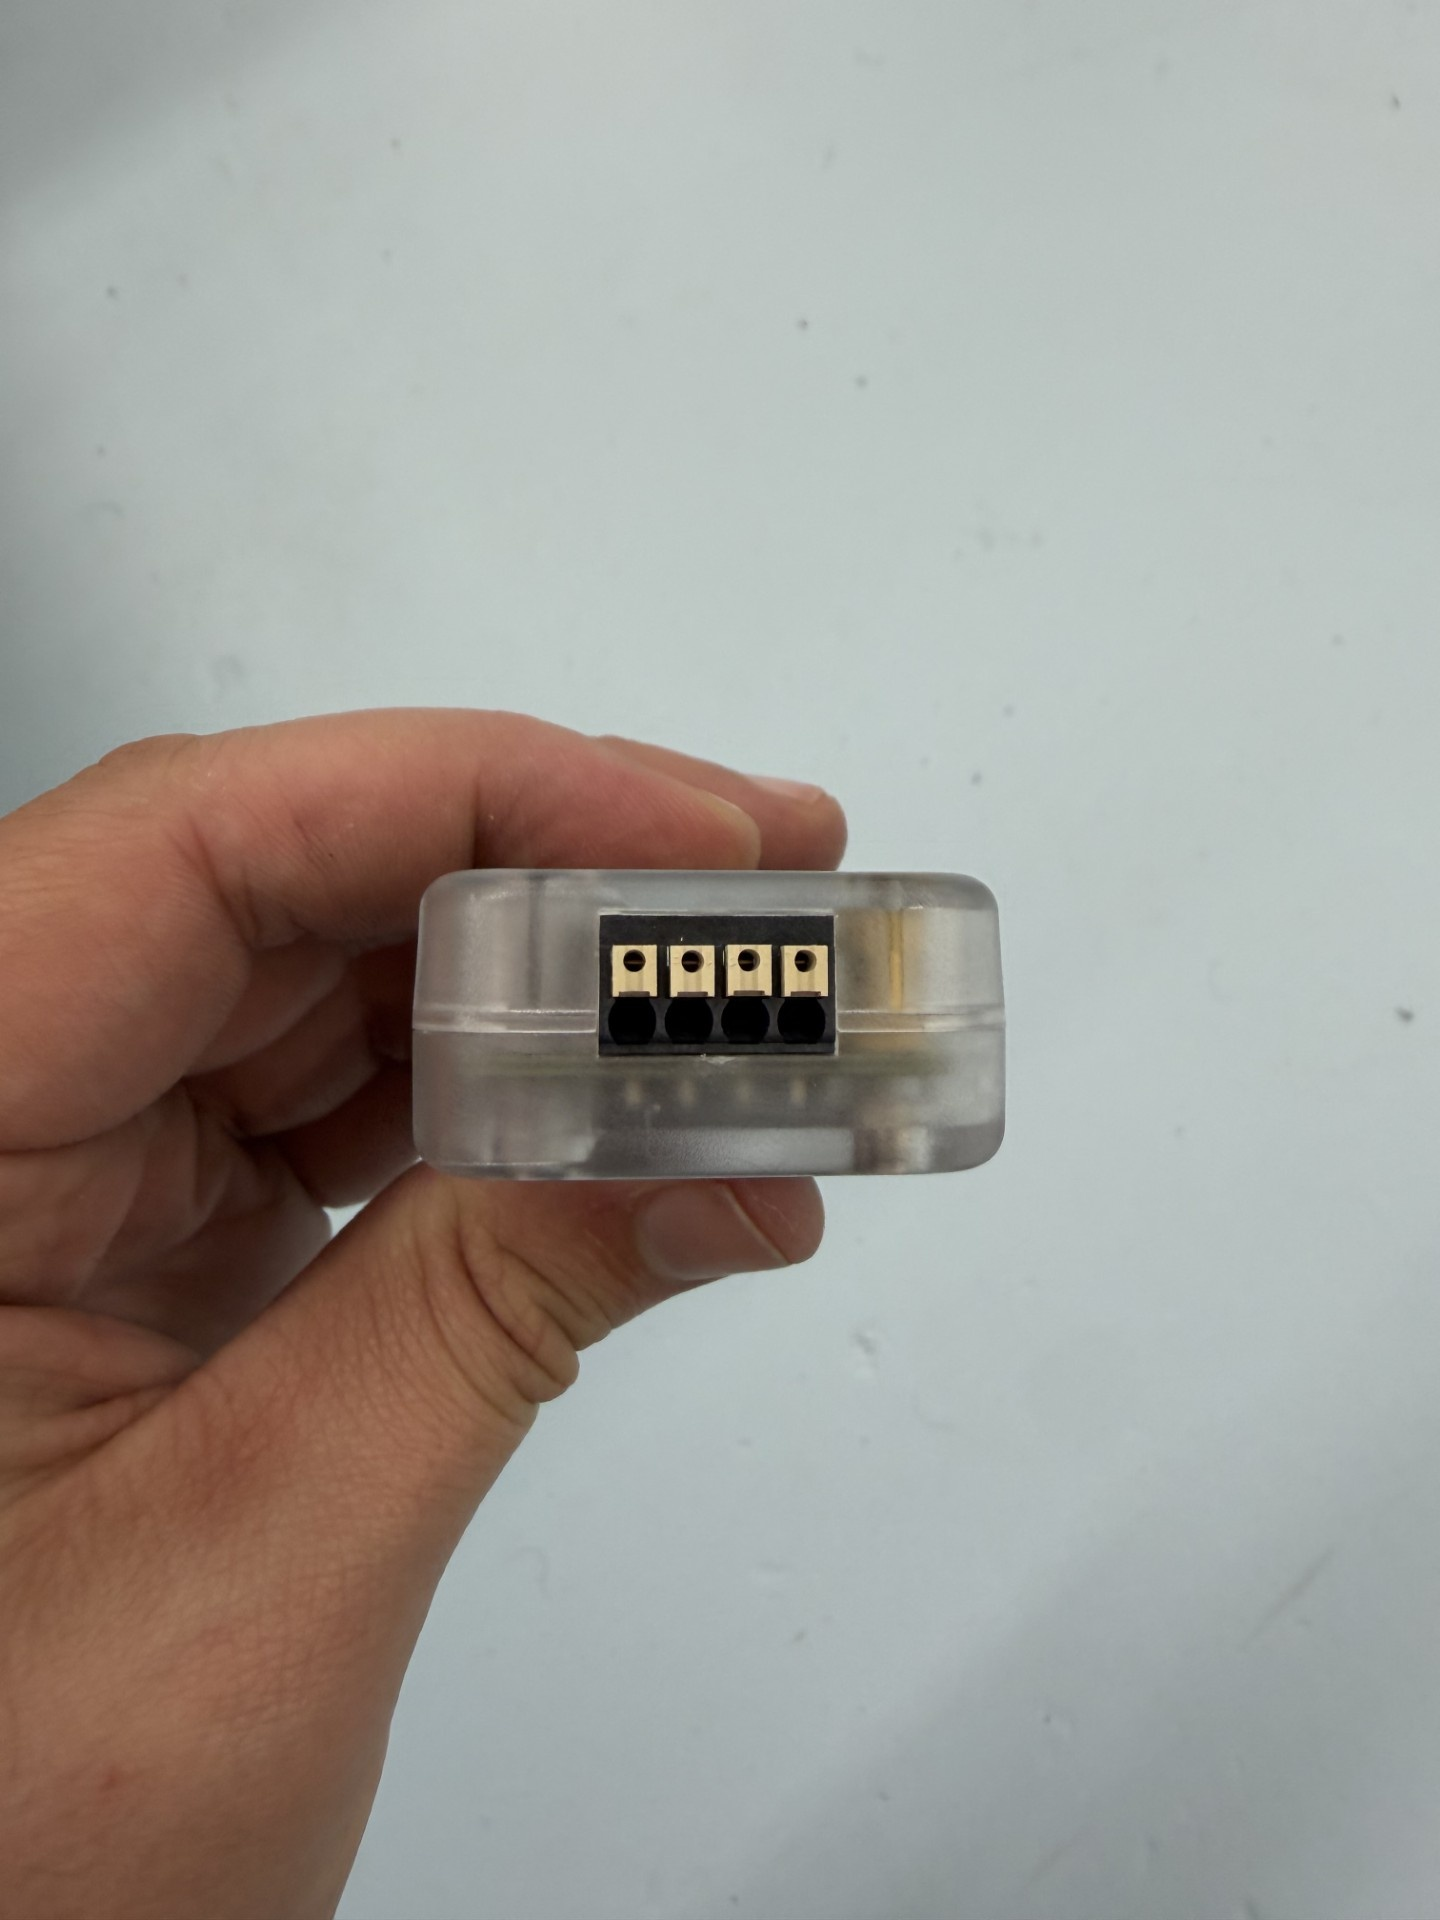
\includegraphics[width=0.47\textwidth]{media/image56.jpeg}
\hfill
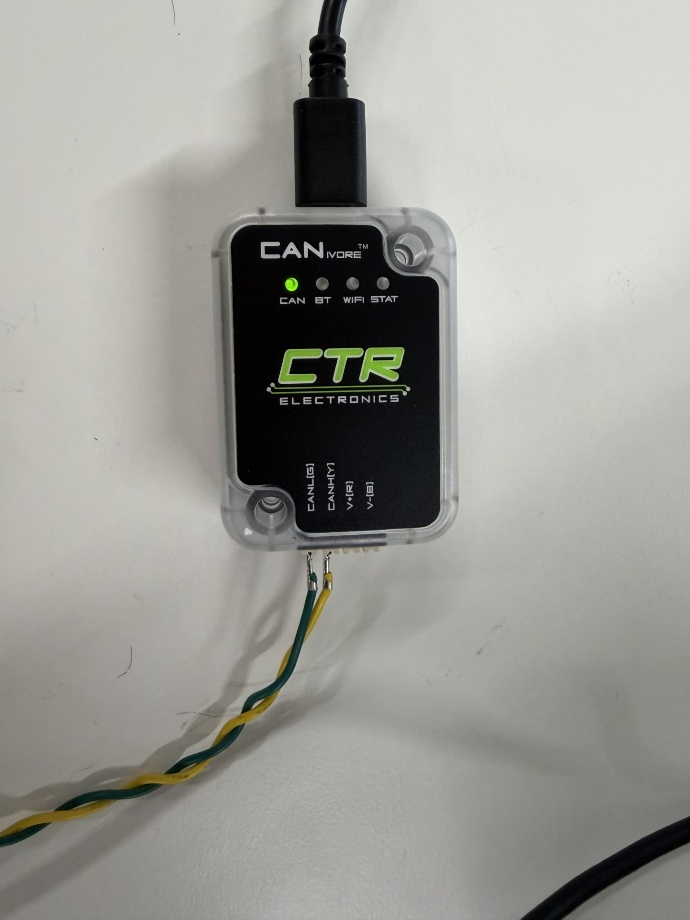
\includegraphics[width=0.47\textwidth]{media/image57.jpeg}
\caption{Inserting the encoder signal wires into the labeled CANivore
slot while pressing the tan button.}
\end{figure}

\assemblystep{Link the Encoders in Series}
Connect the other set of jumper connectors for the same encoder to the
corresponding connectors on the next encoder. Repeat so all 4 encoders
are linked in series.

\begin{figure}[H]
\centering
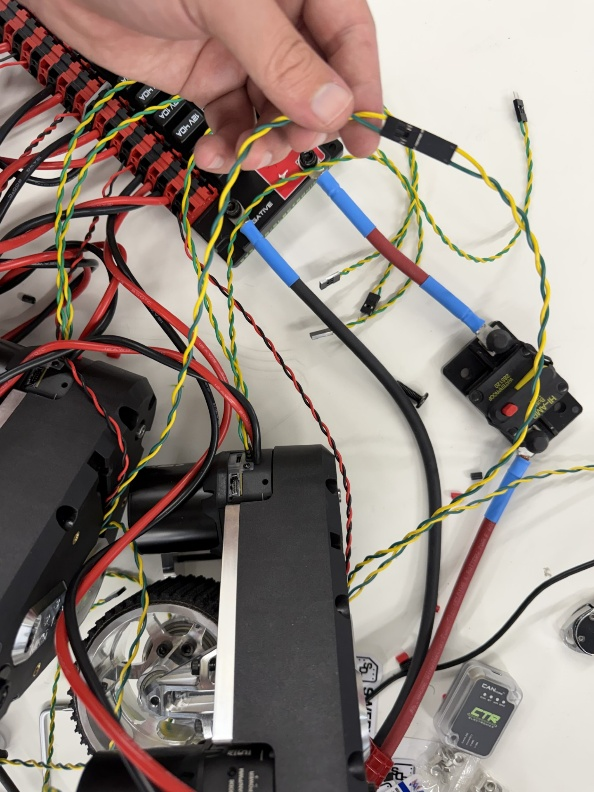
\includegraphics[width=0.5\textwidth]{media/image58.jpeg}
\caption{Jumper connectors linking one encoder to the next, in series.}
\end{figure}

\assemblystep{Configure the CANivore}
Connect the CANivore to a computer via USB-C and launch the Phoenix
Tuner X app. Navigate to the CANivores tab and select the now visible
``Default Name'' item. Here you can rename the device and update the
firmware.

\begin{figure}[H]
\centering
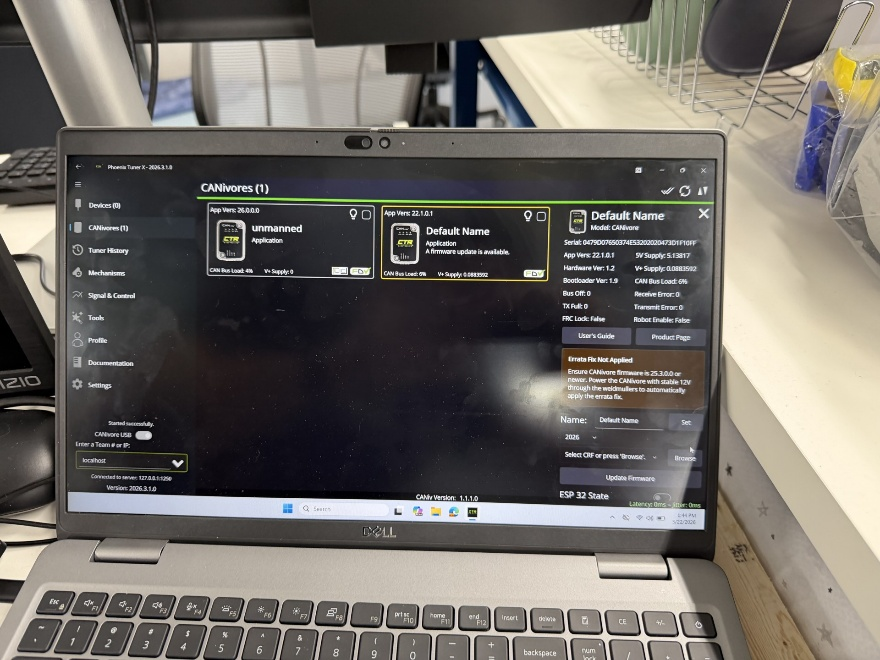
\includegraphics[width=0.5\textwidth]{media/image59.jpeg}
\caption{The CANivore shown under the CANivores tab in Phoenix Tuner~X.}
\end{figure}

\assemblystep{Configure the Encoders}
After updating, an item will be visible in the devices tab. This item
will show that there are 4 devices with this device. When clicked, the
first encoder will appear. Rename the device ID and update the firmware.
In this case, 1-4 was used for the device IDs. Repeat for all encoders
connected to the CANivore.

\begin{figure}[H]
\centering
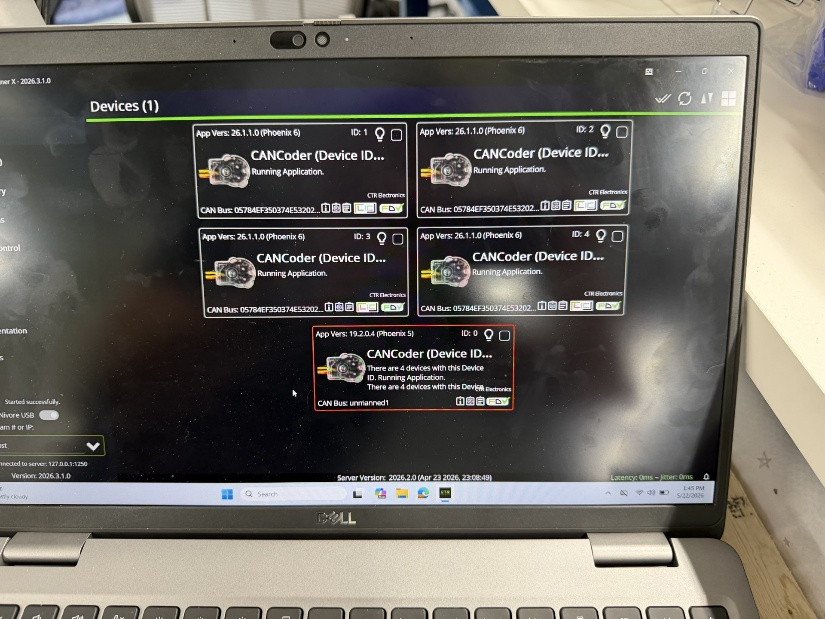
\includegraphics[width=0.47\textwidth]{media/image60.jpeg}
\hfill
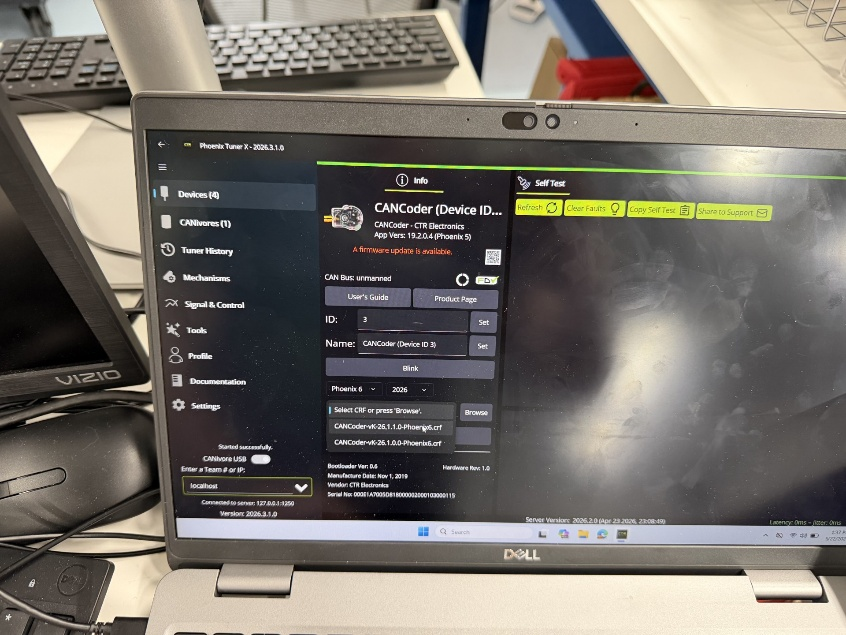
\includegraphics[width=0.47\textwidth]{media/image61.jpeg}
\caption{Renaming each encoder's device ID and updating its firmware in
the devices tab.}
\end{figure}

\assemblystep{Test the Motors}
\begin{figure}[H]
\centering
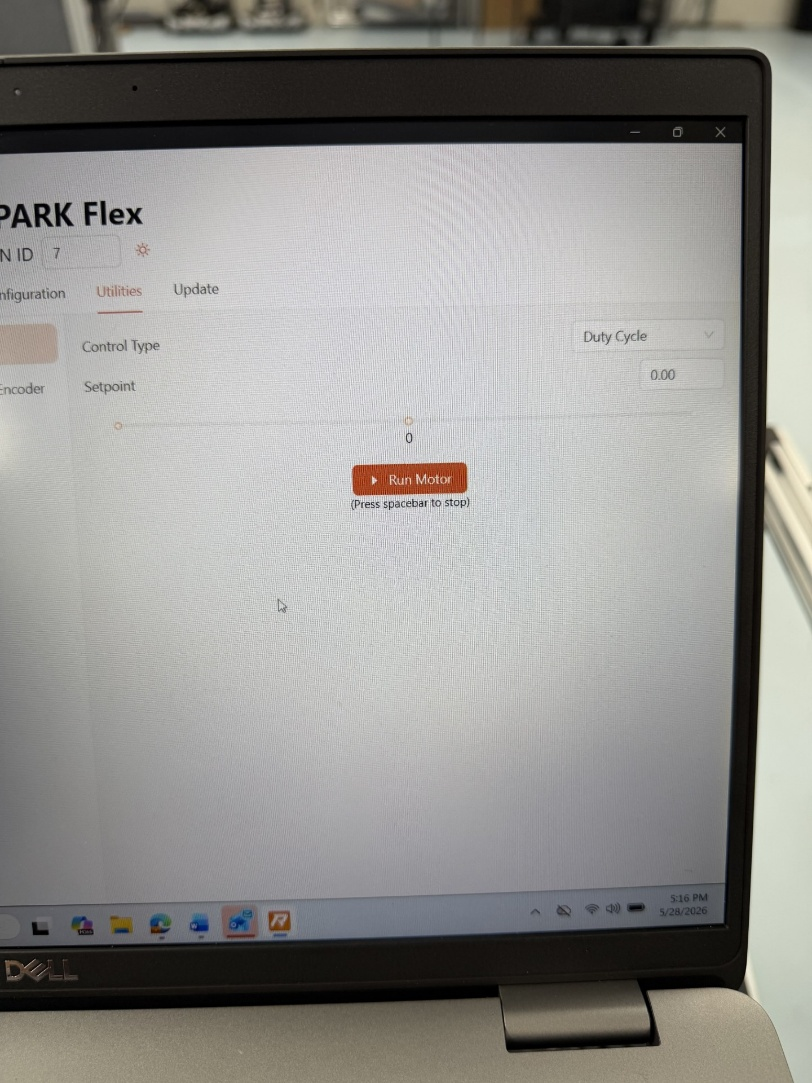
\includegraphics[width=0.5\textwidth]{media/image62.jpeg}
\caption{Running a motor from the Utilities tab to verify drive and steer
movement.}
\end{figure}

Press the yellow lever in to power on the motors. Connect to a motor in
the REV Hardware Client 2 via USB-C. Prop the motor up so that the wheel
is not touching the ground and is clear to turn and rotate. Under the
Utilities tab for the motor, click run motor then change the set point
slightly in both the positive and negative directions. Drive motors
should spin the wheel while steer motors should change the direction.

\begin{tipbox}
Values between .25 and .5 are enough to make the motors spin. Too high
of a set point will make the motor spin rapidly.
\end{tipbox}
